\svnInfo $Id: hardware.tex 75 2008-04-07 13:37:13Z axel $
\chapter{Hardware}
\label{chap:Hardware}

Als vor über 25 Jahren die Grundlagen für das Raytracingverfahren entwickelt wurden, unterschied sich die Hardware auf der diese implementiert wurden stark von den Rechnern die heute zu Verfügung stehen.

Damals war ein Zugriff auf den Hauptspeicher ungefähr so schnell wie die Ausführung einer einfachen Operation. In den letzten Jahrzehnten haben die Hersteller die Frequenz mit der ein Prozessor Operationen ausführen kann immer weiter erhöht. Die Geschwindigkeit mit der Daten aus dem Arbeitsspeicher transportiert werden können hat sich allerdings nicht proportional mitentwickelt.

Dies liegt maßgeblich daran, dass für den Hauptspeicher Speicherbausteine verwendet werden, welche die Daten nicht in ausreichend hoher Geschwindigkeit zur Verfügung stellen können. Die Verwendung schnellerer Bausteine ist prinzipiell möglich, jedoch nicht ökonomisch, da diese Lösungen um Größenordnungen teurer wären, als die eingesetzten.\citep{Drepper07}

Eine Konsequenz dieser Architektur ist, dass Probleme wie das Raytracing nun im Gegensatz zu früher nicht mehr durch die Rechenleistung begrenzt werden, sondern durch die Datenmenge, die in kurzer Zeit zum Prozessor übertragen werden kann.

Natürlich sollte Softwareentwicklung so unabhängig wie möglich von der konkreten Hardware sein. Für interaktives Raytracing auf aktuellen PCs ist es jedoch unumgänglich gewisse Strukturen der Hardware zu kennen und bei der Programmierung zu berücksichtigen.
In diesem Kapitel wird erläutert welche Maßnahmen Hardwarehersteller treffen um das Verhältnis zwischen Prozessor- und Speicherzugriffsgeschwindigkeit zu verbessern und wie dies vom Softwareentwickler unterstützt werden kann. Es ist anzunehmen, dass die vorgestellten Konzepte, wie Caches, mindestens mittelfristig auch weiter bei Prozessoren von Arbeitsplatzrechnern Anwendung finden werden.

\section{Cache}

Das wichtigste Konzept zur Verbesserung der oben beschriebenen Situationen sind Caches. Ein Cache ist ein Datenspeicher der aus Bauteilen besteht die Daten in höherer Geschwindigkeit zur Verfügung stellen können als der Arbeitsspeicher.

Welchen Unterschied die theoretisch optimale Nutzung des Caches macht, zeigt ein kleines Rechenbeispiel aus \cite{Drepper07}:

\begin{quotation}
Angenommen, dass der Zugriff auf den Hauptspeicher 200 Zyklen benötigt und der Zugriff auf den Cache 15. Ein Programm, das auf 100 Datenelemente 100mal zugreift, benötigt 2.000.000 Zyklen für Speicherzugriffe und lediglich 168.500 Zyklen wenn alle Daten gecacht werden können. Dies entspricht einer Verbesserung von 91.5\%.
\end{quotation} 

Da diese Bausteine wesentlich teurer sind als die Hauptspeicherbausteine, fällt der Cache meist mehrere Größenordnungen kleiner aus als der Hauptspeicher (2GB Arbeitsspeicher - 2MB Cache). Da die Datensätze, die heutzutage während des Programmverlaufs verarbeitet werden müssen, viel größer sind als der zur Verfügung stehenden Caches, bedarf es guter Strategien um immer die Daten in den Cache zu laden, die als nächstes benötigt werden. Dadurch, dass parallel zu anderen Operationen des Prozessors Daten aus dem Hauptspeicher in den Cache geladen werden können, ist es möglich die langsamen Hauptspeicher-Zugriffzeiten zu verstecken.

Die im Cache gespeicherten Datensätze besitzen eine gröbere Granularität als die des Arbeitsspeichers. Das liegt zum einen daran, dass die Hauptspeicher-Bausteine effizienter arbeiten wenn mehrere Datenwörter am Stück ausgelesen werden. Zum anderen muss der Cache neben den Daten selbst, auch noch die Adresse der Daten im Arbeitsspeicher halten. Die Adresse jeden adressierbaren Datenwortes, welches im Cache abgelegt wird, zu speichern, wäre ineffizient. Ein unnötig großer Teil des teuren Cachespeichers wäre mit Adressen belegt.
Deswegen ist der Cache in \textit{'Lines'} organisiert, welche größer sind als das kleinste durch den Prozessor adressierbare Datenwort. Um wieviel größer hängt vom konkreten Prozessortyp ab.
Bei der Umsetzung von Cache-Lines wird zusätzlich angenommen, dass Daten auf die kurz hintereinander zugegriffen wird ein \textit{räumlichen Nähe} im Speicher besitzen. Diese Annahme ist durchaus berechtigt, denn für die folgendenen zwei, häufig auftretenden Fälle trifft genau das zu:
\begin{description}
 \item[Zusammengesetzte Datentypen]Oft werden einfache Datentypen zu komplexen, strukturierten Typen zusammengefasst. Diese bilden dann die ``kleinsten'' Einheiten die von vielen Teilen eines Programms verarbeitet werden und damit auch zwischen Hauptspeicher und Prozessor ausgetauscht werden. Durch die Kombination mehrerer Felder kann ein Exemplar schnell auf die Größe einer Cacheline anwachsen. Wird auf die verschiedenen Felder zugegriffen profitiert dies vom Caching, da das ganze Objekt in der entsprechenden Cacheline bereits vorliegt.
 \item[Sequenzen kleiner Datensätze]Ein einzelner Buchstabe einer Zeichenkette belegt nur den Bruchteil einer Cacheline. Für solche kleinen Datensätze kommt es jedoch häufig vor, dass sie in großen, sequentiell gespeicherten Blöcken vorliegen. Zum Beispiel profitiert die sequentielle Ausgabe einer Zeichenkette davon, dass selbst wenn diese nicht im Cache liegt, nach Einlesen des ersten Zeichens, die folgenden Zeichen bereits im Cache liegen werden.
 \end{description}

Die zweite Annahme, nach der Caches gestaltet sind, ist die der \textit{zeitlichen Nähe}. Das heißt, es wird davon ausgegangen, dass Daten auf die vor kurzem zugegriffen wurde, in kurzer Zeit wieder gelesen oder geschrieben werden. Dies trifft ibsbesondere für Programmcode zu. So kann es zum Beispiel passieren, dass innerhalb einer Schleife durch einen Funktionsaufruf immer wieder zu einer bestimmten, entfernten Stelle im Speicher gesprungen wird, um das dort liegende Stück Code auszuführen.
Durch die von-Neumann'sche Rechnerarchitektur, nach der die meisten der Arbeitsplatzrechner entworfen sind, liegen der Programmcode und die Daten gemeinsam im Hauptspeicher. Da die Verarbeitung jedoch verhältnismäßig unabhängig voneinander geschieht, hat es sich als vorteilhaft erwiesen getrennte Caches für Promgrammcode und Programmdaten einzuführen. Dies ermöglicht zusätzlich die Dekodierphase für einen Prozessorbefehl im Cache zu überspringen, indem nach der initialen Ausführung der dekodierte Befehl in den Cache geschrieben wird. \citep{Drepper07}

Sowohl das Cachen von Programmdaten, als auch das Pipelining (siehe unten Abschnitt \ref{sec:branch}) setzen vorraus, dass präzise und möglichst weit im Vorraus vorhergesagt werden kann, welche Daten, beziehungsweise Befehle, geladen werden müssen. Kann dieses nicht gewährleistet werden, kommt es zu so genannten \textit{Pipeline stalls}, das heißt der Prozessor muss unter unter Umständen mehr als 100 Zyklen auf Daten warten und führt während dieser Zeit keine Befehle aus.

Um dies zu vermeiden wird viel Energie in die Optimierung der Vorhersage, welcher Code als nächstes ausgeführt wird, investiert. Die entwickelten Verfahren liefern jedoch nur den vollen Effekt, wenn bei der Softwareentwicklung gewisse Richtlinien beachtet werden, auf die im Folgenden näher eingegangen wird. Allgemein lässt sich die bestmögliche Erfüllung der Annahme der \textit{räumlichen} und \textit{zeitlichen} Nähe als Richtlinie formulieren. Da die Erfüllung, beziehungsweise Verletzung dieser Annahmen jedoch häufig nicht offensichtlich ist, werden im Folgenden ein paar konkretere Richtlinien aufgezeigt.

\section{Richtlinien}

Die folgenden Richtlinien sollen dabei helfen, effizienten Code für aktuelle Arbeitsplatzrechner zu erstellen. Leider stehen diese Richtlinien teilweise im Gegensatz zu denen des allgemeinen Softwaredesigns. Umso wichtiger ist es diese Optimierungen an den relevanten Stellen einzusetzen.
Die Frage, die beim Raytracing am häufigsten beantwortet werden muss, ist die nach dem Schnittpunkt eines Strahls mit der Szenengeometrie. Der Programmcode, der dieses Problem behandelt, wird am häufigsten ausgeführt und stellt deswegen den Fokus für die folgenden Maßnahmen dar. Neben einer kurzen Erläuterung einer Richtlinie wird auch die Anwendung dieser Richtlinie für ein Raytracingprogramm dargestellt.
Für die meisten Richtlinien wird eine Entwicklung in C, beziehungsweise C++ angenommen. Programmiersprachen, die weiter von der Hardware abstrahieren, lassen viele der vorgestellten Maßnahmen nicht zu. Die Implementierung eines so komplexen Systems, wie das eines Raytracers, in Assembler, würde wiederum zu einer unwartbaren Codebasis führen.

\subsection{Kompaktheit}

Die Datenmenge, auf die im Verlauf eines Programms zugegriffen wird, auch als ``working set'' bezeichnet. Passt das \textit{working set} komplett in den Cache, muss zur eigentlichen Laufzeit nicht auf den Hauptspeicher zugegriffen werden. Damit würden auch keine Verzögerungen durch die hohen Zugriffszeiten entstehen.
Üblicherweise, und besonders für das Raytracing, übersteigt der Umfang des \textit{working sets} das Fassungsvermögen des Caches jedoch um mehrere Größenordnungen.

Wird für die Datenstrukturen, die vom Programm verwendet werden, darauf geachtet diese möglichst kompakt zu gestalten, können mehr Datensätze im Cache gehalten werden. Damit wird die Wahrscheinlichkeit eines \textit{Cache-hits} erhöht. Darunter versteht man den Fall, dass ein benötigter Datensatz bereits im Cache liegt und nicht aus dem Hauptspeicher geladen werden muss (im Gegensatz zu einem \textit{Cache-miss}).

Bei der Schnittpunktbestimmung sind die am häufigsten benötigten Datensätze die Knoten einer Beschleunigungsdatenstruktur.
Zur kompakteren Darstellung lassen sich verschiedene Techniken anwenden. Oft kann man mehrere Flags (zum Beispiel ob ein Knoten ein innerer Knoten oder ein Blatt ist) gemeinsam in einem Byte speichern, anstatt für jedes Flag ein einzelnes Feld in der Struktur anzulegen.
Beispiele werden in Kombination mit der Anwendung der in Abschnitt \ref{sec:layout} erläuterten Richtlinien vorgestellt.

\subsection{Ausrichtung}

Durch den Compiler wird die Möglichkeit gegeben Exemplare einer Datenstruktur nur an Adressen ganzzahliger Vielfacher eines wählbaren Wertes zuzulassen. Dies entspricht der Ausrichtung einer Datenstruktur auf ein bestimmtes Raster (4,8,12,16 Bytes etc). Durch eine geschickte Wahl dieses so genannten \textit{Alignments} kann man verhindern, dass ein Datenwort, welches kleiner als eine Cacheline ist, zwei Cachelines überlappt.
Dies ist zum Einen bei einem Cache-Miss vorteilhaft, denn beim Laden der Daten muss lediglich eine Cacheline geladen werden. Gleichzeitig wird lediglich eine andere Cacheline überschrieben - und somit implizit die Wahrscheinlichkeit für einen Cache-hit des in der nicht überschriebenen Cacheline enthaltenen Datensatzes, erhöht.
Zum Anderen haben durch die Ausrichtung die niedrigen Bits eine Adresse eines solchen Datensatzes dann immer den Wert 0. In diesen Bits können wiederum kleinere Werte, wie Flags, gespeichert werden.
Auf der anderen Seite führt ein Alignment, das größer ist als die betreffende Datenstruktur, zu entsprechend viel ungenutztem Speicher. Abbildung \ref{fig:cachelines} zeigt die Konsequenzen unterschiedlicher Ausrichtungen verschiedener Datenstrukturen.

\begin{figure}\centering
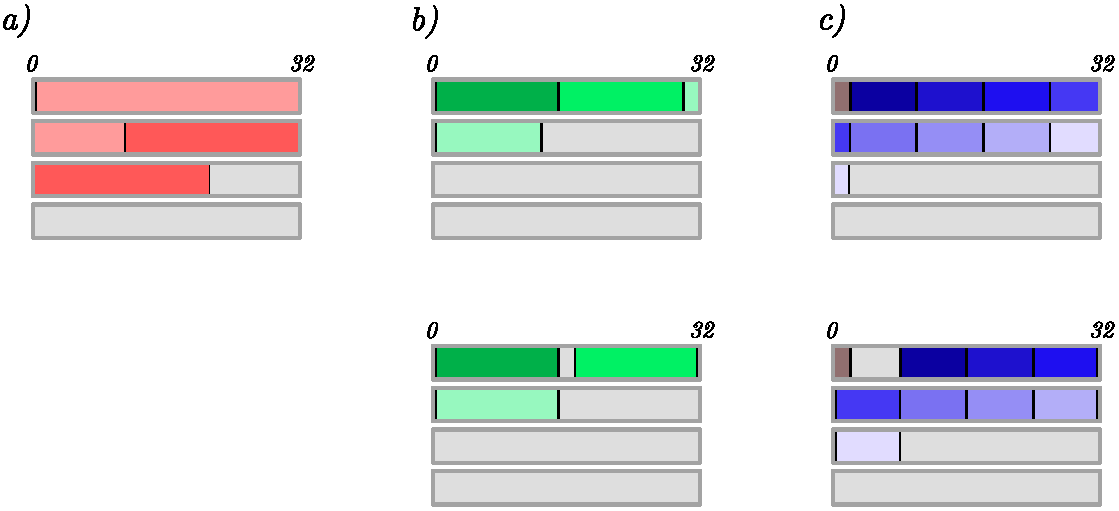
\includegraphics[width=1.0\textwidth]{images/cachelines.pdf} 
\caption[Alignment unterschiedlicher Datenstrukturen]{Alignment unterschiedlicher Datenstrukturen. a) Ein Exemplar ist größer als eine Cacheline. Es kann nicht verhindert werden , dass für ein Element min. zwei Cachelines geladen werden müssen. b) oben: Ein Exemplar belegt 15 Bytes. Durch lückenlose Speicherung beginnt das dritte Element in der ersten und ragt in die zweite Cacheline. unten: Durch ein 16Byte Alignment werden kann die Überlappung verhindert werden, erzeugt aber insgesamt einen wachsenden Speicherbedarf linear zur Menge der gespeicherten Elemente. c) oben: Durch das fehlende Alignment wird hier jedes vierte Element zwei Cachelines überlappen. unten: Durch das 8Byte-Alignment wird nach Daten am Anfang eine 6Byte Lücke erzwungen. Danach können die Datensätze ohne Überlapp und weitere Lücken gespeichert werden.}
\label{fig:cachelines}
\end{figure}


\subsection{Trennung von Daten}
\label{sec:seperatedata}
Um die räumliche Nähe von Daten, auf welche zur gleichen Zeit zugegriffen wird, beizubehalten, müssen manchmal Datenstrukturen aufgetrennt werden. Gibt es Datenfelder, die semantisch zu einem Typ gehören, wovon eines aber besonders häufig gelesen wird, kann es sich lohnen die beiden Datenfelder unabhängig zu speichern. So werden die nicht so häufig gelesenen Felder nicht automatisch mit in den Cache geladen, und es steht mehr Platz für die Daten, auf die öfter zugegriffen wird, zur Verfügung.

Insbesondere gilt dies für Fälle in denen auf ein Feld eines strukturierten Datentypen lediglich lesend zugegriffen wird, während auf einem zweiten Feld häufig schreibende Zugriffe erfolgen. Auch schreibende Zugriffe erfolgen in ganzen Cachelines. Wenn kleine Teile des Inhalts einer Cacheline verändert werden, muss trotzdem die gesamte Cacheline zurück in den Hauptspeicher geschrieben werden. Damit würde die Bandbreite beim Schreiben durch die nicht veränderten Daten unnötig belastet.

Da diese Vorgehen die Komplexität des Programmcodes erheblich erhöhen kann, sei darauf hingewiesen, dass diese Optimierung sich nur in vereinzelten Fällen lohnt. Sie sollte ausschließlich angwendet werden wenn die Größe des \textit{working sets} die des Caches übersteigt, die Daten sequentiell gespeichert werden und auf diese in kritischen Programmabschnitten häufig zugegriffen wird. In keinem Fall sollte dieses Vorgehen zum Regelfall bei dem Entwurf von Datenstrukturen werden.

Ein Beispiel für die korrekte Anwendung dieser Optimierung ist das Mailboxing für disjunkte Raumaufteilungsverfahren. 
Innerhalb eines Frames ändern sich die Geometriedaten nicht. Die Mailboxen einiger Objekte werden unter Umständen jedoch für jeden Strahl verändert. Obwohl die Mailbox semantisch zu dem Objekt gehört, lohnt es sich die Mailboxen gesondert zu speichern. Dadurch kann verhindert werden, dass die Objektdaten, die sich in der selben Cacheline wie die Mailboxingdaten befinden, jedes mal mit in den Hauptspeicher geschrieben werden.

\subsection{Befehlscache}

Wie bereits erwähnt besitzen Prozessoren seit mehreren Jahren getrennte Caches für Programmbefehle und Daten. Die optimale Nutzung des Befehlscaches ist sogar noch wichtiger als die des Datencaches. Wenn der erwartete Programmteil nicht im Cache liegt muss der Prozessor im schlimmsten Fall die Latenz für einen Hauptspeicherzugriff abwarten bis wieder Befehle ausgeführt werden. Eventuelle Latenzen, die sich aus Datencache-misses der enthaltenen Befehle ergeben, addieren sich entsprechend auf.
Da ein Compiler für die letztendliche Codegenerierung zuständig ist, hat der Programmierer meist keinen direkten Einfluss auf die Nutzung des Befehlscaches. Durch die richtige Verwendung des Compilers lässt sich aber indirekt eine bessere Nutzung erreichen.
Generell gilt die Richtlinie der Kompaktheit genauso für den Programmcode wie für die verwendeten Daten.
Die häufigste Quelle für erhöhte Wartezeiten sind Sprünge deren Ziel nicht statisch bestimmbar ist oder deren Ziel
nicht im Befehlscache liegt.

\subsubsection{Inlining}

Daher sollten, besonders bedingte, Sprünge vermieden werden. Um den Sprung in eine entfernte Funktion zu vermeiden bietet der Compiler die Möglichkeit des \textit{Inlining}. Wird eine Methode mit dem Schlüsselwort \verb|inline| gekennzeichnet, ist dies ein Hinweis für den Compiler keine neue Funktion im klassischen Sinne anzulegen, sondern den enthaltene Code direkt an die Stelle des Aufrufs einzufügen. Ob der Hinweis befolgt wird hängt vom jeweiligen Compiler ab, da es sich wie gesagt nur um einen Hinweis handelt.

Die Verwendung von \verb|inline| ist jedoch ein zweischneidiges Schwert. Einerseits spart man einen Funktionsaufruf und die damit verbundenen Kosten. Auf der anderen Seite kann die Menge des Programmcodes stark ansteigen was im Widerspruch zur Richtlinie der Kompaktheit steht. Verschiedene Autoren (\cite{Drepper07}, \cite{Meyers06}) sind sich einig, dass sich Inlining hauptsächlich in zwei Fällen lohnt:
\begin{itemize}
 \item Für sehr kurze Methoden (zum Beispiel Getter und Setter)
 \item Für Methoden die nur einmal aufgerufen werden.
\end{itemize}

Für alle anderen Fälle sollte \verb|inline| nur im Zusammenhang mit genauem Profiling verwendet werden, weil der Code unübersichtlicher und das Debuggen erschwert wird. Im schlechtesten Fall kann die Verwendung von  \verb|inline| sogar Leistungeinbußen mit sich bringen.

Da für die meisten Compiler das Inlining in der Kompilierungsphase geschieht, muss die Funktionsdefinition auch in der Headerdatei vorgenommen werden, was wie bereits angedeutet, die Lesbarkeit herabsetzten kann. Um die Lesbarkeit so wenig wie möglich zu verschlechtern sollten die mit \verb|inline| markierten Methoden außerhalb der Klassendeklaration implementiert werden (siehe Quelltext \ref{inline}).

\begin{lstlisting}[float,belowcaptionskip=8pt,caption={[Sinnvoller Einsatz von inlining]links: Definition aller Inlinemethoden mindert Lesbarkeit. rechts: Getrennte Definition der Methoden macht Schnittstelle der Klasse klar erkennbar},label=inline]
         class BadStyle {                          class GoodStyle {
           public:                                    public:
             void methodA();                            void methodA()
             inline void methodB() {                    void methodB();
               doSomething();                           void methodC();
             }                                     }
             void methodC();                       // Ende der Klassen Deklaration
         }                             
                                                   inline void GoodStyle::methodB() {
                                                      doSomething();
                                                   }
\end{lstlisting}

\subsubsection{Dynamische Bindung}

In C++ gibt es die Möglichkeit Methoden mit dem Schlüsselwort \verb|virtual| zu markieren. Dadurch wird dem Entwickler ermöglicht eine polymorphe Klassenhierarchie zu implementieren. 
Da die Sprungadresse virtueller Methoden aber erst zur Laufzeit berechnet wird, sollte auf die Verwendung in kritischen Programmteilen verzichtet werden. Für das Raytracing heißt das konkret, dass in der Phase der Schnittpunktbestimmung keine virtuellen Methoden aufgerufen werden sollten. \cite{Wald04} berichtet, dass der Aufruf einer einzigen virtuellen Methode einen Leistungseinbruch von 5\% zur Folge hatte.

Da die Verwendung von virtuellen Methoden maßgeblich zu einer guten Programmstruktur beiträgt, sei auch hier nochmal darauf hingewiesen, dass solche Maßnahmen ausschließlich in leistungskritischen Programmabschnitten anzuwenden sind.


\subsubsection{Pipeline stalls}
\label{sec:branch}

Da die Prozessoren aber selbst schneller als die Cachezugriffe sind, wird zur Befehlsverarbeitung das so genannte Pipelining angewendet. Hierbei wird die Ausführung eines Befehls in Teilphasen zerlegt. Diese bestehen zum Beispiel aus einer Phase zum Laden des Befehls und einer zum Dekodieren. Dazu kommen weitere Phasen zum Laden der Operatoren, die Verarbeitung und das Speichern der Ergebnisse (\cite{RechPom}). Durch parallele Ausführung der einzelnen Phasen unterschiedlicher Befehle lassen sich die Latenzen für das Laden einzelner Befehle verstecken (siehe Abbildung \ref{fig:pipeline}).

Als Beispiel nehmen wir eine vierstufige Pipeline an, von der jede Stufe zur Ausführung einen Takt benötigt. Für die Ausführung wird also jeder Befehl in vier Phasen zerlegt, die jeweils einen Takt dauern. Ein Befehl hat somit eine \textit{Latenz} von vier Takten. Die sequentielle Ausführung von vier Befehlen würde 16 Takte dauern. Jede Phase wird von einem eigenständigen Modul ausgeführt.
Dadurch wird es möglich, unterschiedliche Phasen aufeinander folgender Befehle parallel auszuführen. Der \textit{Durchsatz} von Befehlen kann so deutlich erhöht werden. Für das Beispiel der vierstufigen Pipeline heißt das, dass die vier Befehle, anstatt in 16, in lediglich 7 Takten ausgeführt werden können.

\begin{figure}\centering
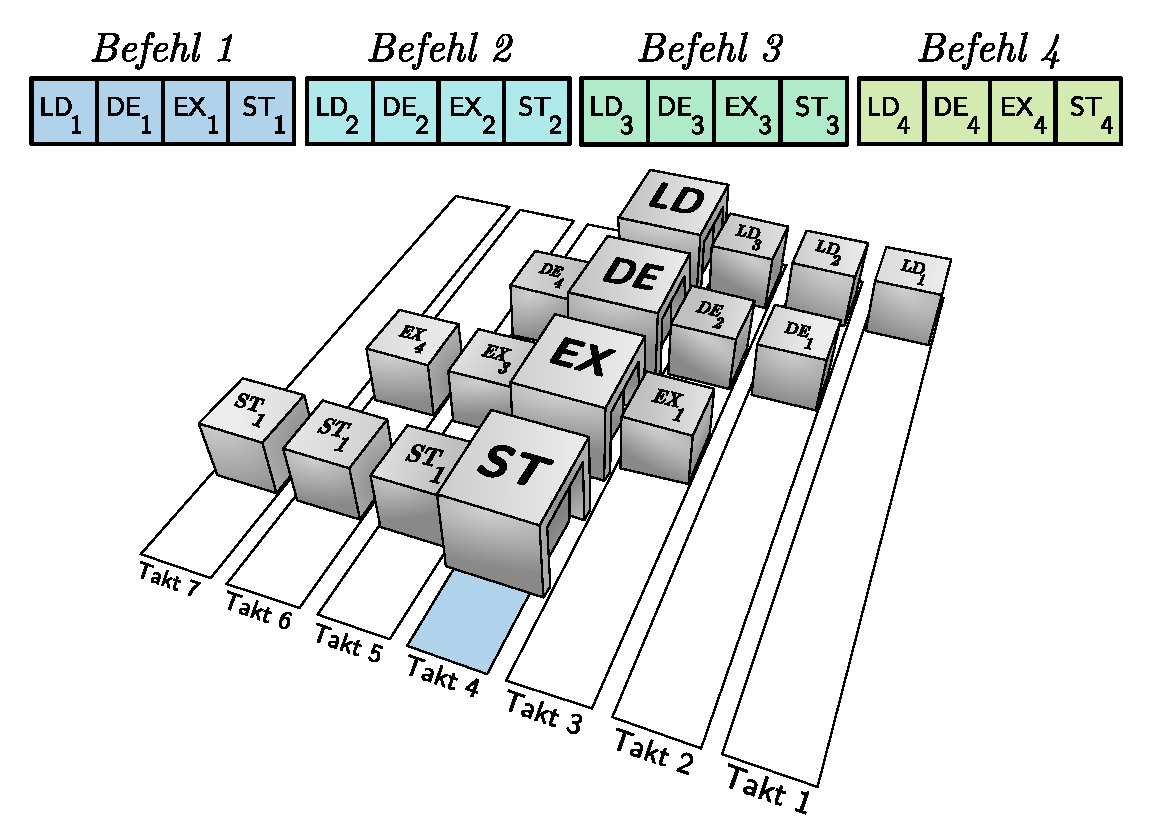
\includegraphics[width=0.7\textwidth]{images/pipeline.pdf} 
\caption[Vierstufiges Pipelining]{oben:Jeder Befehl wird in vier Phasen zerlegt. unten: Durch parallele Ausführung verschiedene Phasen unterschiedlicher Befehle ($LD_4, DE_3, EX_2, ST_1$) lässt sich der Durchsatz erhöhen \footnotesize{(LD = Befehl laden, DE = dekodieren, EX = Ausführen, ST = Speichern}}
\label{fig:pipeline}
\end{figure}

Das Pipelining liefert aber nur den vollen Durchsatz, wenn die Pipeline die ganze Zeit gefüllt bleibt. Nach einem bedingten Sprung können zwei verschiede Folgen von Befehlen ausgeführt werden. Die Befehlspipeline kann aber lediglich eine Folge aufnehmen. Eine falsche Vorhersage führt dazu, dass die bereits in der Pipeline vorhandenen Befehle ungültig sind. Für diesen Fall muss die Pipeline komplett geleert werden. Der volle Durchsatz kann erst wieder erreicht werden, wenn der erste Befehl alle Stufen der Pipeline durchlaufen hat.
Diese so genannte \textit{misprediction penalty} kann aufgrund der unterschiedlichen Länge der Pipeline bei verschiedenen Prozessoren von 12 bis über 50 Takte umfassen \cite{Fog08ASM}. Dies ist zwar nicht so verheerend wie eine schlechte Ausnutzung des Caches, aber trotzdem signifikant an den kritischen Stellen eines Programms.
Die Hardwarehersteller verwenden dementsprechend viel Kapazitäten, um eine gute Sprungvorhersage zu erreichen. Solange die Verzweigungen regelmäßigen Mustern folgen funktioniert diese recht gut.
Trotzdem ist die einfachste Methode falsche Vorhersagen zu vermeiden, in kritischen Abschnitten so wenig Verzweigungen wie möglich zu verwenden.

\subsection{Rekursion gegenüber Iteration}

Die iterative Formulierung eines Algorithmus arbeitet meist effizienter als die rekursive Variante, da letztere zusätzliche Funktionsaufrufe benötigt (\cite{Lantzman07}).
Deswegen bietet es sich an, kritischen, rekursiven Code, wie zum Beispiel die Traversierung der Raumaufteilungshierarchie, dementsprechend umzuformulieren (\cite{Wald04}).

\section{Effiziente Speicherauslegung}
\label{sec:layout}
Besonders wichtig für eine effiziente Berechnung der Schnittpunkte der Strahlen mit der Szenengeometrie ist eine höchst effiziente Implementierung der Beschleunigungsdatenstruktur. Mindestens genauso wichtig wie die eigentlichen Berechnungen ist dabei die Auslegung der Struktur im Speicher. Für hierarchische Strukturen besteht diese zum Einen daraus, wie ein einzelner Konten ausgelegt ist, und zum Anderen wie die verschiedene Knoten relativ zueinander im Speicher angeordnet sind. Im Folgenden werden Optimierungen für \textit{binäre} Bäume erläutert.

\subsection{Allokation und Anordnung}

Die Speicherung von Daten in einem Baum ist zwar \textit{logisch} nicht linear, wird dies physikalisch aber spätestens beim Speichern im \textit{linearen} Arbeitsspeicher.
Durch die verschiedenen Möglichkeiten die Hierarchie im linearen Speicher anzuordnen ergeben sich mehr oder weniger geeignete Strukturen. Besonders was die effiziente Cachenutzung betrifft kann es hier zu signifikanten Leistungsunterschieden kommen.

Bei der klassischen Top-down Konstruktion wird der Speicher während der Konstruktion für jeden Knoten einzeln angefordert. Der Elternknoten speichert dann zwei Referenzen auf die ihm folgenden Teilbäume (Abbildung \ref{fig:memlayout} a)).
Eine erste Optimierung für binäre Bäume ist das Speichern der zwei Kindknoten direkt hintereinander. Da von der Adresse des ersten Kindknotens, durch einfache Inkrementierung auf die Adresse des zweiten Knotens geschlossen werden kann, erübrigt sich eine explizite Speicherung der zweiten Adresse (Abbildung \ref{fig:memlayout} b)).
Alternativ kann auch einer der Kindknoten direkt nach dessen Elternknoten gespeichert werden. Auch hierbei kann auf die explizite Adressierung dieses Kindknotens verzichtet werden. Befürworter der zweiten Strategie argumentieren, dass es hier bei der Traversierung eine höhere Wahrscheinlichkeit gibt, dass der nächste zu traversierende Kindknoten bereits mit dem Elternknoten zusammen in den Cache geladen wurden (Abbildung \ref{fig:memlayout} c)).

\begin{figure}\centering
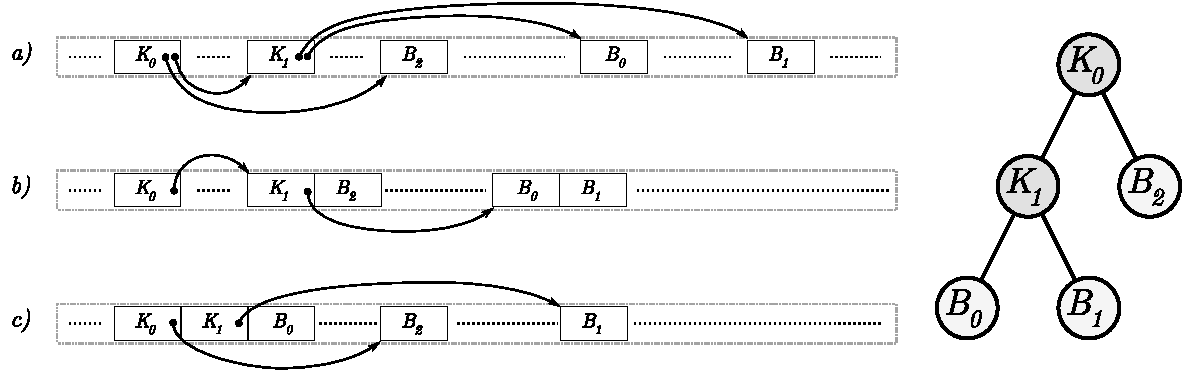
\includegraphics[width=1.0\textwidth]{images/memlayout.pdf} 
\caption[Speicherauslegung für binären Baum]{Drei Möglichkeiten den rechts gezeigten Baum im Speicher abzulegen. a) Die Implementierung mit zwei Zeigern pro innerem Knoten benötigt den meisten Platz und eine möglichst große Entfernung zu den Kindknoten, welches die Wahrscheinlichkeit eines Cache-miss erhöht. b) Das Speichern der Kinder direkt hintereinander ermöglicht eine schlankere Darstellung. Falls beide Teilbäume traversiert werden müssen besteht eine erhöhte Wahrscheinlichkeit, dass der zweite Knoten einen Cache-hit erzeugt. Für Bäume, die größer als die Cache sind, tritt dies in den oberen Ebenen selten ein, da die Cacheline sehr wahrscheinlich schon ersetzt wurde. c) Die Auslegung im Speicher belegt den gleichen Platz. Allerdings gibt es eine 50/50 Chance, dass der Kindknoten, der jetzt direkt auf den aktuellen Knoten folgt, als nächstes traversiert wird und somit einen Cache-hit erzeugt.}
\label{fig:memlayout}
\end{figure}

\subsection{Kompakte Knotendarstellung}

\begin{lstlisting}[belowcaptionskip=8pt,float,mathescape=true,caption={[Kompakte Speicherauslegung eines Bounding Intervall Hierarchy Knotens]BIH Knoten wie durch Waechter beschrieben. Belegt auf einer 32Bit Archtiktektur lediglich 12Byte entspr. 16Byte auf 64Bit Hardware},label=src:bihnode]
typedef struct {
 longIndex;// lowest bits:axis(00, 01, 10) or leaf(11)
 union {
   long     Items ;  // leaf only
   float    Clip[2]; //internal node only
 };
} BIH_Node ;
\end{lstlisting}

Für eine cacheeffiziente Implementierung müssen die Knoten besonders kompakt gespeichert werden. In \cite{Benthin06} wird ein effizientes Layout für einen kd-tree Knoten vorgestellt (siehe Quelltext \ref{src:kdnode}).\classref{accelleration}{KdNode}Ein gleichermaßen effizientes Layout für einen BIH-Knoten wird in \cite{BIH06} vorgestellt (siehe Quelltext \ref{src:bihnode}).\classref{accelleration}{BihCompact} Für beide Auslegungen wird angenommen, dass lediglich ein Kindknoten eines inneren Knoten explizit referenziert werden muss. Anstatt die Unterscheidung zwischen einem Blatt und einem inneren Knoten, wie in der objektorientierten Programmierung üblich, durch dynamische Bindung umzusetzen, wird explizit ein entsprechendes Flag gespeichert. So kann während der Traversierung vollkommen auf die Verwendung virtueller Methoden verzichtet werden.

\begin{lstlisting}[belowcaptionskip=8pt,float,mathescape=true,caption={[Kompakte Speicherauslegung eines kd-Tree Knotens]kd-tree Knoten in einem acht Byte Layout nach Benthin bzw Wald (ausgehend von 32-Bit Architektur). Verschiedene Attribute werden durch effiziente logische Anweisungen in einem unsigned int kombiniert},label=src:kdnode]
// efficient 8-byte layout for a kd-Tree node
struct KDTreeNode {
  union
  {
    float split_position; // position of axis-aligned split plane
    unsigned int items;   // or number of leaf primitives
  }
  unsigned int dim_offset_flag;
  // the 32 bits of 'dim_offset_flag' are used to encode multiple data
  // bits[0..1]  : encode the split plane dimension
  // bits[2..30] : encode an address offset
  // bit[31]     : encodes whether a node is an inner node or a leaf
};
// macros for extracting node information
#define ISLEAF(n)    (n->dim_offset_flag & (unsigned int)(1<<31))
#define DIMENSION(n) (n->dim_offset_flag & 0x3)
#define OFFSET(n)    (n->dim_offset_flag & 0x7FFFFFFC)
\end{lstlisting}

\subsubsection{Fortgeschrittene Speicherauslegung}
\label{sec:toxiememlayout}
\cite{WK07} stellen einen Konstruktionsalgorithmus für hierarchische Beschleunigungsdatenstrukturen vor, welcher die Anforderungen an ein effizientes Speichermanagement, für aktuelle Hardware erfüllt. Das Vorgehen ist sowohl für Verfahren, die den Raum disjunkt teilen, als auch für Verfahren, welche die Objektmenge partitionieren, geeignet.
Das Verfahren nimmt eine Top-down-Konstruktion vor, welche durch Einführung eines neuen Terminierungskriteriums in einem festen Speicherblock auageführt werden kann. Dadurch kann der benötigte Speicher \textit{einmalig} angefordert werden und weitere Allokationsaufrufe sind überflüssig. Das Verfahren ist mit jeder Heuristik zur Wahl der Partitionierung einsetzbar. 

Die Vorgehensweise wird in Abbildung \ref{fig:memrt} für die dort dargestellte Szene veranschaulicht. Die Eingabe für den Algorithmus ist die Größe des Speicherblocks und der Zeiger auf den Speicherblock. Die Indizes zu den im Voxel enthaltenen Objekte befinden sich am Anfang des Blocks.
Dabei werden die folgenden Schritte ausgeführt:
\begin{enumerate}
 \item Das erste Element befindet sich links von der Trennebene und verbleibt auf seiner Position. Der Zeiger für das nächste zu bearbeitende Element wird inkrementiert.
 \item Das zweite Element liegt vollständig hinter der Trennebene. Der Index wird an das Ende des Block geschrieben.
 \item Das letzte Element der noch nicht untersuchten Objekte wird an die frei gewordene Stelle bewegt.
 \item Das Objekt fünf überlappt beide Voxel. Der Bereich für Elemente, die in beide Voxel reichen, befindet sich direkt vor dem Bereich der Objekte, die ausschließlich im rechten Voxel liegen.
 \item Der Zeiger für das nächste zu bearbeitende Element wird nicht weiterbewegt. Das Objekt, welches sich als letztes in der Liste der noch nicht untersuchten Objekte befindet, wird an die frei gewordene Stelle bewegt.
 \item Auch das Objekt vier ragt in beide Voxel und wird an den Anfang des Bereichs für doppelt referenzierte Objekte bewegt.
 \item Das letzte nicht klassifizierte Objekt in der Liste wird wieder an die Stelle des Zeigers für das nächste zu bearbeitende Element bewegt.
 \item Das aktuell zu untersuchende Objekt drei befindet sich vollständig hinter der Trennebene. Um für dieses Element Platz zu schaffen wird das letzte Element aus der Liste der doppelt referenzierten Objekte, an den Anfang dieser Liste bewegt.
 \item Das Objekt drei wird an den frei gewordenen Platz verschoben. Dort ist jetzt der neue Anfang für die Liste der Objekte, die ausschließlich im rechten Voxel liegen. Es sind keine weiteren Objekte in der Liste der nicht klassifizierten Objekte zu finden. Der Sortiervorgang ist abgeschlossen.
 \item Die Elemente der Liste der doppelt referenzierten Objekte wird an das Ende der Objekte, die sich vollständig vor der Trennebene befinden kopiert.
 \item Um für den aktuell zu erzeugenden inneren Knoten Platz zu schaffen werden so viele Objekt vom Anfang der linken Liste an deren Ende verschoben, dass am Anfang genug Platz für einen Knoten entsteht.
 Der freie Bereich zwischen den beiden Listen ist der Speicher, der beiden Teilbäumen gemeinsam zur Verfügung steht, um den Raum weiter aufzuteilen. Er wird proportional zu den, in den Teilbäumen enthaltenen, Objekten aufgeteilt. 
Der Speicherplatz für die beiden Kindknoten selbst, wird aber zuvor davon abgezogen, da dieser auf jeden Fall für jeden der Teilbäume zur Verfügung stehen muss.
 \item Die Liste der Objekte für den rechten Teilbaum wird nun um die Menge des dem rechten Teilbaum zugeteilten freien Speichers nach vorne verschoben.
\end{enumerate}
\srcref{accelleration}{KdTreeBase}{subdivide}
\begin{figure}\centering
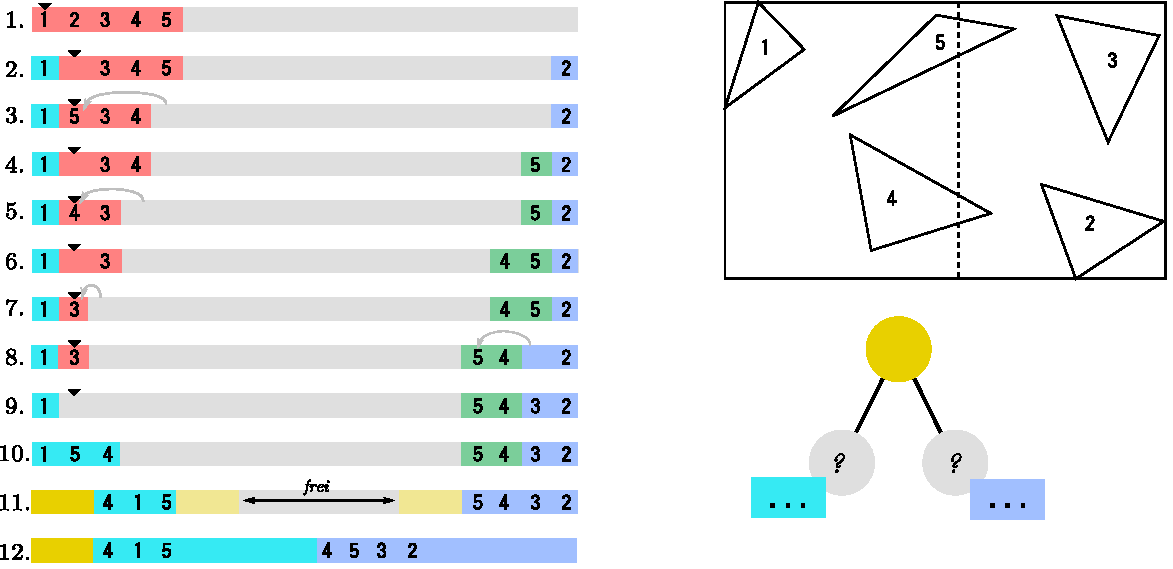
\includegraphics[width=1.0\textwidth]{images/memrt.pdf} 
\caption[Konstruktion eines Binärbaums im einem begrenzten Speicherblock]{Vorgehensweise bei der Top-down-Konstruktion in einem festen Speicherblock nach \cite{WK07}}
\label{fig:memrt}
\end{figure}

Danach kann das Verfahren für die beiden eingezeichneten Teilblöcke von vorn begonnen werden. Das neue Terminierungskriterium ergibt sich aus der Menge des freien Speichers. Verbleibt nicht genügend Speicher, um die beiden entstehenden Teillisten und jeweils einen Knoten zu speichern, wird am Anfang des Speicherblocks ein Blattknoten erzeugt auf den die Eingabeliste von Objekten folgt. Diese muss zu diesem Zweck vor der Sortierung gesichert werden.
Für Verfahren bei denen die Objektliste partitioniert wird entfällt der Teil für die Behandlung von mehrfach referenzierten Objekten.

Die Auslegung der Knoten, die sich durch diese Art der Konstruktion ergibt, ist damit ähnlich wie in Abbildung \ref{fig:memlayout} c). Zusätzlich folgt die Liste der Objekte in einem Blattknoten direkt auf diesen Blattknoten. Dies begünstigt den Zugriff über einen Cache. Auch hierfür wird bei der klassischen Top-down Konstruktion, zumindest für kd-trees, meistens dynamisch Speicher angefordert.
Das \textit{lazy building} lässt sich intuitiv mit dem beschriebenen Vorgehen verbinden. Der einzigen Nachteil ist, dass Teile des einmal reservierten Speichers unter Umständen nicht genutzt werden.

Einen weiteren Vorteil dieser Art den Baum zu konstruktion, den \cite{WK07} aufzeigen, ist die Möglichkeit verschiedene Baumtypen zu mischen. So lassen sich durch das Hinzufügen eines weiteren Flags beispielsweise kd-Tree Knoten mit BIH Knoten mischen. Dies ermöglicht die effizientere Behandlung von leerem Raum in einer BIH. Wird bei der Konstruktion festgestellt, dass ein Teilbaum keine Objekte enthält kann anstatt einer Neupositionierung der Trennebene wie in \ref{constrbih} vorgeschlagen, ein kd-Tree Knoten angelegt werden. Dieser würde den leeren Raum effizienter behandeln als die reine Verwendung der BIH.

\section{Parallelisierung}

Parallelisierung lässt sich mit aktuellen Arbeitsplatzrechnern auf zwei unterschiedlichen Ebenen sinnvoll realisieren: zum Einen auf Befehlsebene, zum Anderen auf Threadebene. Die beiden Ansätze stehen orthogonal zueinander und können somit beide gleichzeitig eingesetzt werden, um die Gesamtleistung zu erhöhen.

\subsection{SIMD}

SIMD\abbrev{SIMD}{Single Instruction Multiple Data} steht für \textit{Single Instruction Multiple Data}. Ursprünglich nur Großrechnern vorbehalten besitzt inzwischen nahezu jeder Prozessor eines Arbeitsplatzrechners diese Technologie. Es handelt sich dabei um die Fähigkeit, die gleiche Operation auf Vektoren von Daten parallel auszuführen.
Die Befehle sind in eigenen Befehlssätzen beschrieben und arbeiten in aktuellen Architekturen auf anderen Registern als die normalen Befehle. Aktuelle Arbeitsplatzrechner unterstützen die Bearbeitung von 128Bit Registern. Der Befehlssatz, der hierfür hauptsächlich genutzt wird, ist der SSE(2)-Befehlssatz, da dieser auf vielen Rechnern zur Verfügung steht. Auf den momentan verbreitetsten Prozessoren von AMD und Intel stehen acht 128Bit Register dafür zu Verfügung, auf den aktuelleren Modellen bereits 16 \cite{AMD06}, 
\abbrev{SSE}{Streaming SIMD Extensions}
\cite{Intel08}.

Die für das Raytracing interessante Interpretation der 128Bit stellen vier Gleitkommazahlen einfacher Genauigkeit dar. 
Der SSE Befehlssatz bietet arithmetische, logische und bitweise Operatoren die unter anderem auf Vektoren von vier Gleitkommazahlen angewendet werden können. Ein typisches Beispiel ist die Addition von vier Paaren von Gleitkommazahlen (Abbildung \ref{fig:sseadd}). 

\begin{figure}\centering
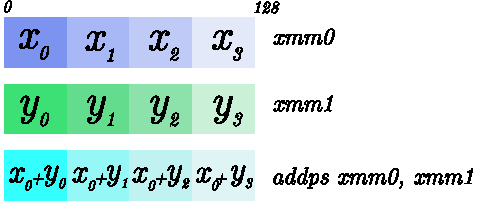
\includegraphics[width=0.4\textwidth]{images/sse1.pdf} 
\caption[SSE Beispiel: Addition]{Mit Intels SSE Befehlssatz können kann mit einer einzigen Anweisung eine Operation auf vier unabhängigen Operanden(-paaren) ausgeführt werden.}
\label{fig:sseadd}
\end{figure}

Für die Verwendung der SSE Befehle ergeben sich zwei Ansätze. Der erste Ansatz versucht, eine Operation auf einem Operandenpaar eines komplexen Datentyps, durch die Verwendung der SSE Befehle, zu beschleunigen. Die Organisation der Daten erfolgt in Feldern von strukturierten Datentypen - so genannten \abbrev{AoS}{Arrays of structures}Arrays of structures(AoS). Da beim Raytracing besonders viele Probleme der räumlichen Geometrie gelöst werden müssen, bietet sich der dreidimensionale Vektor als Kandidat für eine effizientere Verarbeitung mit SSE an. 
Die Operationen für 3D-Vektoren lassen sich leicht kapseln. Eine effizientere Implementierung dieser Operationen durch SSE-Befehle hätte den Vorteil, dass diese für Rest des Programms transparent wäre.
Ein Beispiel für eine solche Operation ist die bereits vorgestellte Addition (Abbildung \ref{fig:sseadd}). Ein Nachteil dieses Ansatzes ist, dass sich die vektorisierte Verarbeitung nur dort effizient einsetzen lässt, wo die Operationen unabhängig auf den Komponenten des Vektors arbeiten. Für Operationen wie das Kreuzprodukt bietet diese Art der Implementierung mit SSE nicht den optimalen Durchsatz, da die Komponenten nicht voneinander unabhängig verarbeitet werden können. Einen weiteren Nachteil stellt die Tatsache dar, dass für \textit{dreidimensionale} Vektoren nur drei Viertel des 128Bit Registers genutzt werden, was eine weitere Verschlechterung gegenüber der idealen Auslastung darstellt.

\begin{lstlisting}[belowcaptionskip=8pt,float,caption={[\textit{Structure of arrays Anordnung} im Vergleich zum \textit{Array of structures}]Die Anordnung der Daten im "Structure of arrays"-Layout ermöglicht eine  effizientere Nutzung des SSE Befehlssatzes},label=src:aosvssoa]
   // Array of structures                // Structure of arrays
   typedef struct {                      typedef struct {
     float x,y,z;                            float x[NumOfVertices];
   } Vector3;                                float y[NumOfVertices];
                                             float z[NumOfVertices];
   Vector3 vertices[NumOfVertices]       } VertexList;
                                         VertexList vertices
\end{lstlisting}

Die Alternative ist die Anordnung der Daten in einer so genannten \textit{Structure of Arrays}(SoA)\abbrev{SoA}{Structure of Arrays}. Für die Speicherung von geometrischen Vektoren im SoA Format werden die Komponenten verschiedener Vektoren in einem gemeinsamen Feld abgelegt. Quelltext \ref{src:aosvssoa} zeigt die unterschiedlichen Auslegungen im direkten Vergleich.
Durch die SoA Auslegung wird es möglich, statt einzelne Schritte einer Operation, die gesamte Operation parallel auszuführen. Für das Vektorbeispiel heißt das: Anstatt die Operationen auf den Komponenten zu parallelisieren, wird die gesamte Operation für vier Vektoren, beziehungsweise Vektorpaare, ausgeführt. Dies behebt die beiden Schwächen des AoS Formats. Die Anzahl der parallelisierbaren Operationen hängt nun nicht mehr von der Anzahl der Komponenten des Vektors ab. Die Operationen für eine Komponente werden jetzt für vier Vektoren gleichzeitig ausgeführt. Damit werden auch \textit{horizontale}, also Operation die auf verschiedenen Komponenten zweier Vektoren arbeiten, möglich.
Aus diesen Gründen ermöglicht die SoA-Auslegung eine effizientere Nutzung der SIMD Kapazitäten eines aktuellen Prozessors als die AoS-Auslegung (\cite{IntelOpt07}).

\subsubsection{Parallele Traversierung}

\cite{Wald04} beschreibt in seiner Arbeit die effiziente Verfolgung von vier kohärenten Strahlen. Mit Hilfe des SSE Befehlssatzes werden vier Strahlen gleichzeitig durch einen kd-Tree verfolgt. Die Traversierungsroutine muss hierfür entsprechend angepasst werden. Dabei wird wie bereits in Abschnitt \ref{sec:kdpacket} vorgegangen: Jeder Teilbaum, der von mindestens einem Strahl geschnitten wird, wird weiter untersucht. Strahlen die lediglich einen Teilbaum besuchen, weil ein Nachbarstrahl dessen Voxel schneidet, werden maskiert um zu verhindern, dass diese Strahlen die Traversierung weiterer Teilbäume auslösen.
\cite{Benthin06} beschreibt eine erweiterte Implementierung die den SSE Befehlssatz verwendet um größere, kohärente Strahlpakete zu verfolgen. Dabei setzt er ein von \cite{Reshetov05} erstmals beschriebenes Verfahren ein, um Teilbäume für das gesamte Paket von der Traversierung auszuschließen, ohne dass die konkret im Paket enthaltenen Strahlen bekannt sein müssen. Wie auch in Kapitel \ref{sec:packets} beschrieben, wird stellvertretend ein Pyramidenstumpf betrachtet. Durch Intervallarithmetik ist es möglich, über die Extremwerte des Schnitts des Pyramidenstumpfes mit der Trennebene, darauf zu schließen, welcher Teilbaum traversiert werden muss. Die Grundidee der Intervallarithmetik ist es, die gängigen Operationen, die in der klassischen Arithmetik auf individuellen Werten ausgeführt werden, auf Intervalle auszudehnen. Ein gute und knappe Einführung wird von \cite{BWS06} gegeben.

Für Strahlpakete, die sich aus Kacheln der Projektionsebene ergeben, können wieder die vier ``Eck-Strahlen'' als Repräsentanten des Pyramidenstumpfes verwendet werden. Wie in Abbildung \ref{fig:frustum} dargestellt, lassen sich die Minima, beziehungsweise Maxima der Schnittpunkte mit der Trennebene verwenden, um zu bestimmen welcher Teilbaum traversiert werden muss.
Die Bestimmung der vier Schnittpunkte ist ein idealer Kandidat für die parallele Implementierung mit dem SSE Befehlssatz. Für eine effiziente Lösung müssen (mindestens) die vier Eckstrahlen im SoA-Format gespeichert werden. Eine entsprechende Auslegung eines Strahlpakets könnte wie in Quelltext \ref{src:rapacket} aussehen.

\begin{lstlisting}[float,label=src:rapacket,caption=Definition einer Datenstruktur für Strahlpakete im SoA-Format]
typedef struct {
  float origin_x[4];
  float origin_y[4];
  float origin_z[4];

  float direction_x[4];
  float direction_y[4];
  float direction_z[4];
} RayQuadruple;
\end{lstlisting}

Auch der Schnittest von Strahlpaketen und Objekten lässt sich durch die Verwendung der SSE Befehle effizienter gestalten. In \ref{sec:packets} wurde bereits das Verfahren von \cite{DHS04} angesprochen. Es verwendet die Eck-Strahlen eines Pakets, um einen konservativen, schnellen Test zu implementieren mit dem sich feststellen lässt, ob das Dreieck überhaupt von dem Paket geschnitten werden kann. Da die Tests auch hier für vier Strahlen unabhängig voneinander ausgeführt werden müssen, ist eine parallele Implementierung mittels SIMD nur konsequent.

Kann nicht ausgeschlossen werden, dass ein Strahl das Dreieck schneidet, müssen alle Strahlen des Pakets auf Schnitt getestet werden. Für größere Pakete lohnt es sich die enthaltenen Strahlen wiederum in 2x2 Paketen und im SoA-Format anzuordnen. Diese können dann mit dem gleichen Algorithmus, parallel getestet werden.


\begin{figure}\centering
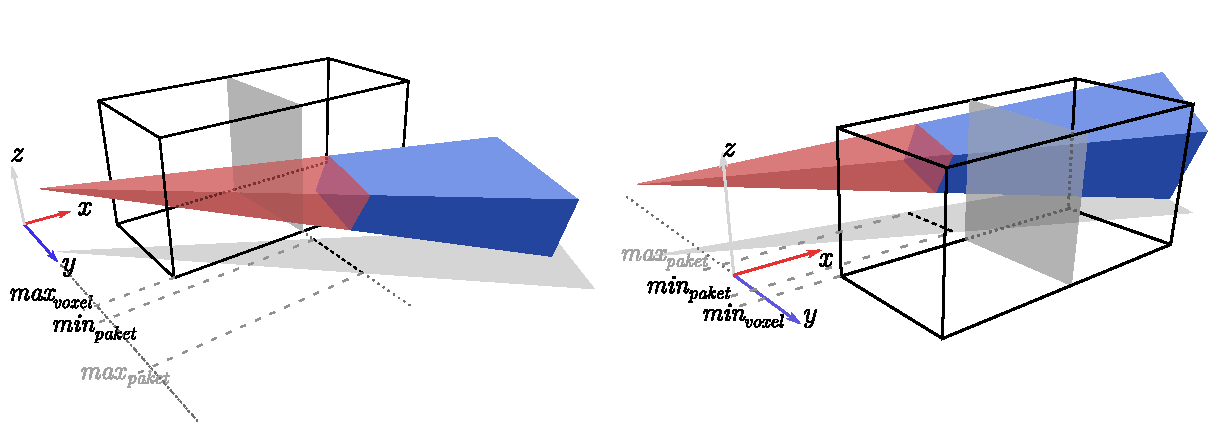
\includegraphics[width=1.0\textwidth]{images/frustum.pdf} 
\caption[Inverse Frustum culling]{Unter der Annahme, dass der aktuelle Voxel von dem Frustum geschnitten wird, gilt: Liegt das Minimum des Intervalls hinter dem Maximum der Trennebene wird lediglich der vordere Voxel geschnitten. Liegt das Maximum des Frustums vor dem Minimum der Trennebene wird ausschließlich der hintere Voxel geschnitten. Bei negativer Ausbreitungsrichtung sind die beiden Fälle genau vertauscht. Tritt keiner der beiden Fälle ein müssen beide Teilbäume traversiert werden. Der Test muss immer für die beiden Achsen ausgeführt werden die parallel zur Trennebene liegen}
\label{fig:frustum}
\end{figure}

\subsubsection{Parallele Konstruktion}

Ein Schritt der bei fast allen Konstruktionsalgorithmen häufig ausgeführt wird, ist die Bestimmung auf welcher Seite einer Ebene ein Objekt liegt, beziehungsweise ob es die Ebene schneidet. Hier gibt es zwei Möglichkeiten diese Operation durch SIMD effizienter zu gestalten.
\begin{description}
 \item[Ein Objekt vier Ebenen] Müssen mehrere Kandidaten von Ebenen verglichen werden kann der Test eines Objekts durch die Verwendung von SIMD mit mehreren Ebenen gleichzeitig durchgeführt werden.
 \item[Eine Ebene mit vier Objekten]Alternativ lässt sich auch eine Ebene parallel mit vier Objekten testen. Die Objekte, beziehungsweise die AABBs, müssen für eine effiziente Umsetzung im \textit{SOA} Format gespeichert werden.
 \end{description}
Welches Verfahren die höhere Leistung liefert hängt von dem eingesetzten Konstruktionsalgorithmus ab. Neben der Tatsache, dass vier Rechenoperationen gleichzeitig ausgeführt werden, wird besonders für den ersten Ansatz auch eine bessere Nutzung des Caches erreicht. Für den parallelen Test mit vier Ebenen muss ein Objekt lediglich einmal aus dem Hauptspeicher geladen werden.

\subsubsection{Paralleles Shading}

Eine allgemeine Parallelisierung der Shadingberechnungen ist nicht möglich. Da Programmcode für die Nutzung von SIMD besondere Befehle (zum Beispiel SSE) verwenden muss, ist es unabdingbar, jeden Shader einzeln für die parallele Verarbeitung anzupassen. Dies ist besonders anspruchsvoll für Anwendungen in denen die Shader durch den Benutzer zur Laufzeit gestaltet werden können.

Der gängige Ansatz besteht daraus, vier Schnittpunkte eines Strahls mit der Geometrie gleichzeitig zu \textit{shaden}. Der Shader bezeichnet den Algorithmus, der bestimmt, wieviel von dem eintreffenden Licht an einem Punkt im Raum in Richtung der Kamera reflektiert wird. Für die Unterstützung mit SIMD wird er so angepasst, dass er vier Punkte gleichzeitig verarbeiten kann.
Welcher Shader ausgeführt wird hängt von dem Material des Objekts ab, das der Primärstrahl geschnitten hat. Die Schnittpunkte, die als Ergebnis einer Traversierung mit SIMD Befehlen entstehen, liegen meist bereits im \textit{SoA}-Format vor (welches nun auch für den Shadingalgorithmus benötigt wird). Da ein Shader jedoch lediglich für \textit{ein} Material verwendet werden kann, ist der parallele Shadingalgorithmus lediglich dann anwendbar, wenn alle Schnittpunkte den gleichen Shader verwenden. Insbesondere für kohärente Strahlpakete ist die Wahrscheinlichkeit jedoch hoch, dass dies der Fall ist.
Für Pakete, die Schnittpunkte mit Objekten unterschiedlicher Materialien enthalten, muss entweder die nicht parallele Version des Algorithmus verwendet werden oder für die unterschiedlichen Shader werden solange Schnittpunkte ``gesammelt'' bis genügend für die Ausführung der parallelen Version zur Verfügung stehen. Der letztere Ansatz erfordert jedoch zusätzlich die Verfolgung, welcher Schnittpunkt zu welchem Bereich auf der Projektionsfläche gehört.

\begin{figure}\centering
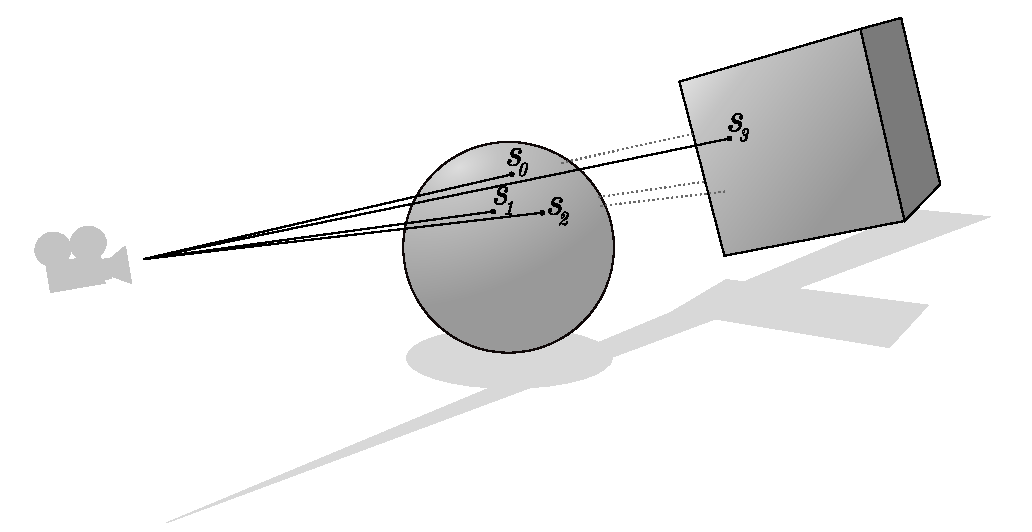
\includegraphics[width=0.6\textwidth]{images/simdshade.pdf} 
\caption[Strahlpaket schneidet unterschiedliche Objekte]{Der Schnittpunkt $S_3$ liegt auf einem anderen Objekt als die anderen drei Schnittpunkte. Parallelisierung mit SIMD kann nur angewendet werden, wenn die Kugel und der Würfel den gleichen Shader verwenden.}
\label{fig:simdshade}
\end{figure}


\subsection{Multithreading}

Um die Rechenleistung eines Rechners zu steigern wird in aktuellen Prozessoren die Anzahl der enthaltenen Rechenkerne erhöht und nicht mehr die Pipeline verlängert. Die verschiedenen Kerne bekommen dabei teilweise eigene Caches und teilen sich die höheren Caches. Abbildung \ref{fig:cpumem} zeigt eine typische Anordnung. Um den Zustand des Speichers, der in den verschiedenen Caches der Kerne repräsentiert wird, konsistent zu halten, wird ein vierstufiges Protokoll genutzt. Dieses Protokoll bewirkt unter anderem, dass wenn ein Kern eine Cacheline verändert, die Cachelines der anderen Kerne, welche den gleichen Speicherbereich abbilden, als ungültig markiert werden. Dadurch werden sie automatisch beim nächsten Zugriff neu geladen.
Um den Synchronisationsaufwand, welcher durch die Verwendung von mehreren Kernen entsteht, so gering wie möglich zu halten ist darauf zu achten, dass unterschiedliche Threads nicht auf den selben Speicherbereich zugreifen, wenn einer der Zugriffe schreibend ist. Auch hierfür ist die Trennung von Daten, die ausschließlich gelesen werden, von solchen, die wiederholt geschrieben werden, wichtig (siehe auch Abschnitt \ref{sec:seperatedata}).
Durch die Verwendung des Schlüsselwortes \verb|const| ist der Compiler in der Lage, entsprechende Variablen zu erkennen und von den anderen Variablen getrennt zu speichern (\cite{Drepper07}).

\begin{figure}\centering
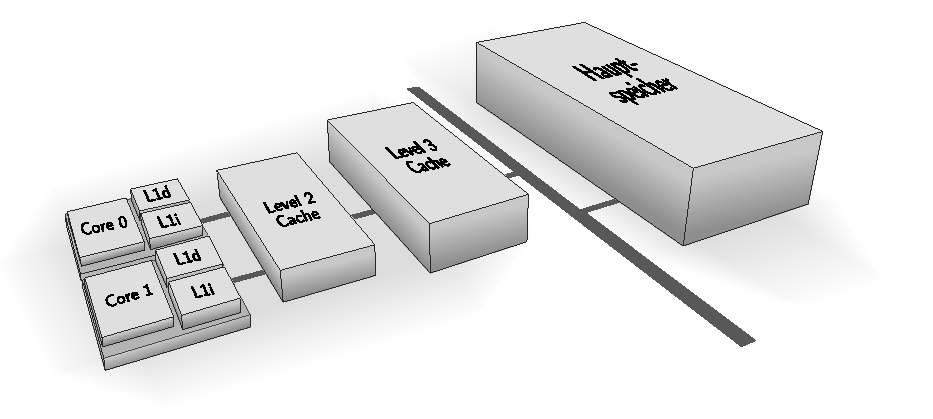
\includegraphics[width=0.7\textwidth]{images/cpumem.pdf} 
\caption[Typische Cachestruktur aktueller Prozessoren.]{Typische Cachestruktur aktueller Prozessoren. Die Abbildung zeigt einen Prozessor mit zwei Kernen. Jeder Kern verfügt über einen eigenen Level 1 Befehls-(L1i) und Datencache(L1d). Die Caches der höheren Level werden von beiden Kernen gemeinsam genutzt.}
\label{fig:cpumem}
\end{figure}

\subsubsection{Parallele Traversierung}

Die Parallelisierung der Traversierung durch Threads ist im Vergleich zu SIMD verhältnismäßig einfach. Jedem Thread werden Bereiche der Projektionsfläche zugewiesen, die dieser zu rendern hat. Diese sollten nicht zu wenig Strahlen enthalten, da sonst der Aufwand die Threads zu administrieren größer wird als der Leistungsgewinn. Sind die Kacheln hingegen zu groß kann dies dazu führen, dass ein Thread seinen Bereich viel schneller abgearbeitet hat als andere. Sind keine ungerenderten Kacheln mehr vorhanden muss der Thread warten bis die anderen Threads ihre Arbeit beendet haben.

Für den Traversierungsvorgang an sich ist es günstig, wenn die Bereiche der verschiedenen Threads nah beieinander liegen, da die Threads dann ähnliche Knoten der Beschleunigungsstruktur besuchen, und diese in den gemeinsamen Cacheebenen eher Cache-hits erzeugen. Andererseits ist es dann auch wahrscheinlicher, dass sich einige der Cachelines des Framebuffers in die geschrieben wird überlappen. Um dies zu verhindern, bieten sich folgende drei Möglichkeiten an:
\begin{enumerate}
 \item Die Kacheln verschiedener Threads in getrennten Regionen starten
 \item Die Framebufferinhalte in getrennte Speicherbereiche schreiben und später zusammenfügen
 \item Bei der Kacheleinteilung die Cachelinebreite beachten, sodass eine Kachelkante immer an einer Cacheline beginnt beziehungsweise endet.
\end{enumerate}

\subsubsection{Parallele Konstruktion}

Der einfachste Weg mehrere Threads bei der Konstruktion einer hierarchischen Bechleunigungsdatenstruktur einzusetzen, ist jedem Thread die Konstruktion einzelner Teilbäume zu überlassen. Voraussetzung hierfür ist, dass genügend unabhängige Teilbäume zur Verfügung stehen. Dies ist besonders für den Wurzelknoten nicht gegeben. Eine effiziente Nutzung aller Kerne kann also erst geschehen, wenn die obersten Ebenen der Hierarchie konstruiert wurden.

Alternativ kann zunächst eine grobe Vorsortierung in so genannte \textit{``Bins''} vorgenommen werden. Hierfür wird der Raum der Szene entlang einer Achse in diskrete Raumelemente aufgeteilt und jedes Objekt, je nach Überlappung, einem oder mehreren dieser Voxel zugeordnet. BVH und BIH profitieren dabei davon, dass jedes Objekt lediglich einmal referenziert wird.
Für die Zuordnung wird die Liste der Objekte in genau so viele Partitionen aufgeteilt, wie es Threads gibt. Danach untersucht jeder Thread die Objekte einer Partition und weist sie dem entsprechenden \textit{Bin} zu.
Um zu verhindern, dass es zu Schreibkonflikten, beziehungsweise hohem Synchronisationsaufwand zwischen den Threads kommt, schreibt jeder Thread in einen eigenen Satz von \textit{Bins}. Nachdem alle Threads die Klassifizierung der Objekte beendet haben, werden die \textit{Bin}-Sätze der verschiedenen Threads zusammengeführt.\citep{Wald07}

Eine weitere Alternative, die Konstruktion von BVHs mit Threads zu parallelisieren, welche ebenfalls von \cite{Wald07}  vorgeschlagen wird, wählt die \textit{Bins} in Form eines dreidimensionalen, gleichmäßigen Gitters. Die Gitterzellen lassen sich durch Berechnung der AABBs der enthaltenen Objekte und paarweiser Kombination mit den Nachbarzellen zu einer gültigen BVH zusammenführen. Die Zellen, die nun noch mehrere Objekte enthalten, können wiederum parallel weiter durch unterschiedliche Threads unterteilt werden. Alternativ können sie erst in der Traversierungsphase bei Bedarf konstruiert werden (vgl. Abschnitt ``Schnelle Konstruktion'' \ref{sec:lazy}).

